Komprimeringsalgoritmen "Huffman coding", er udviklet af David A. Huffman. Huffman udviklede algoritmen mens han var Ph.D studerende på MIT. I 1952 udgav han dokumentet"A Method for the Construction of Minimum-Redundancy Codes"\cite{A_Method_for}. Her beskrev Huffman hvordan hans komprimerings algoritme fungerede. Hvad han havde udviklet, var en 'lossless' (tabsfri) komprimerings metode, hvilket betyder, at der ikke vil være noget tab af information ved at komprimere. Komprimeringsmetoden er beregnet til binære systemer, og formålet med algoritmen er at få en given datamænde til at benytte et minimalt antal bit. 

For så at kunne få de orginale data tilbage fra den komprimerede form, kræver det selvfølgelig, at man har en form for ordbog, der beskriver hvilke tegn, der hører sammen med hvilke bits.

For at Huffman coding effektivt kan fungere, skal algoritmen have adgang til hele datamængden, for at kunne analysere hyppigheden af forskellige tegn. Dette betyder at algoritmen skal løbe i gennem datamængden to gange. Første gang, for at indsamle statistik, og anden gang for så at foretage den reelle komprimering. En eksempel på en algoritme der ikke har den ulempe er komprimeringsmetoden "Lempel-Ziv-Welch".

Figur \ref{fig:huffmantree} viser et Huffman træ, genereret ud fra sætningen "this is an example of a huffman tree" \cite{huff_wiki}. Tabel \ref{tab:huffmantable} viser frekvensen, og en kort kode i bits for de forskellige tegn. Nu fylder sætningen kun 135 bits, mod de 288 bits sætningen originalt fyldte - en besparelse på ca 53\%. Denne kræver selvfølgelig, at de binære koder allerede er kendes af algoritmen der skal dekomprimere datamængden.

\begin{figure}[H]
\centering
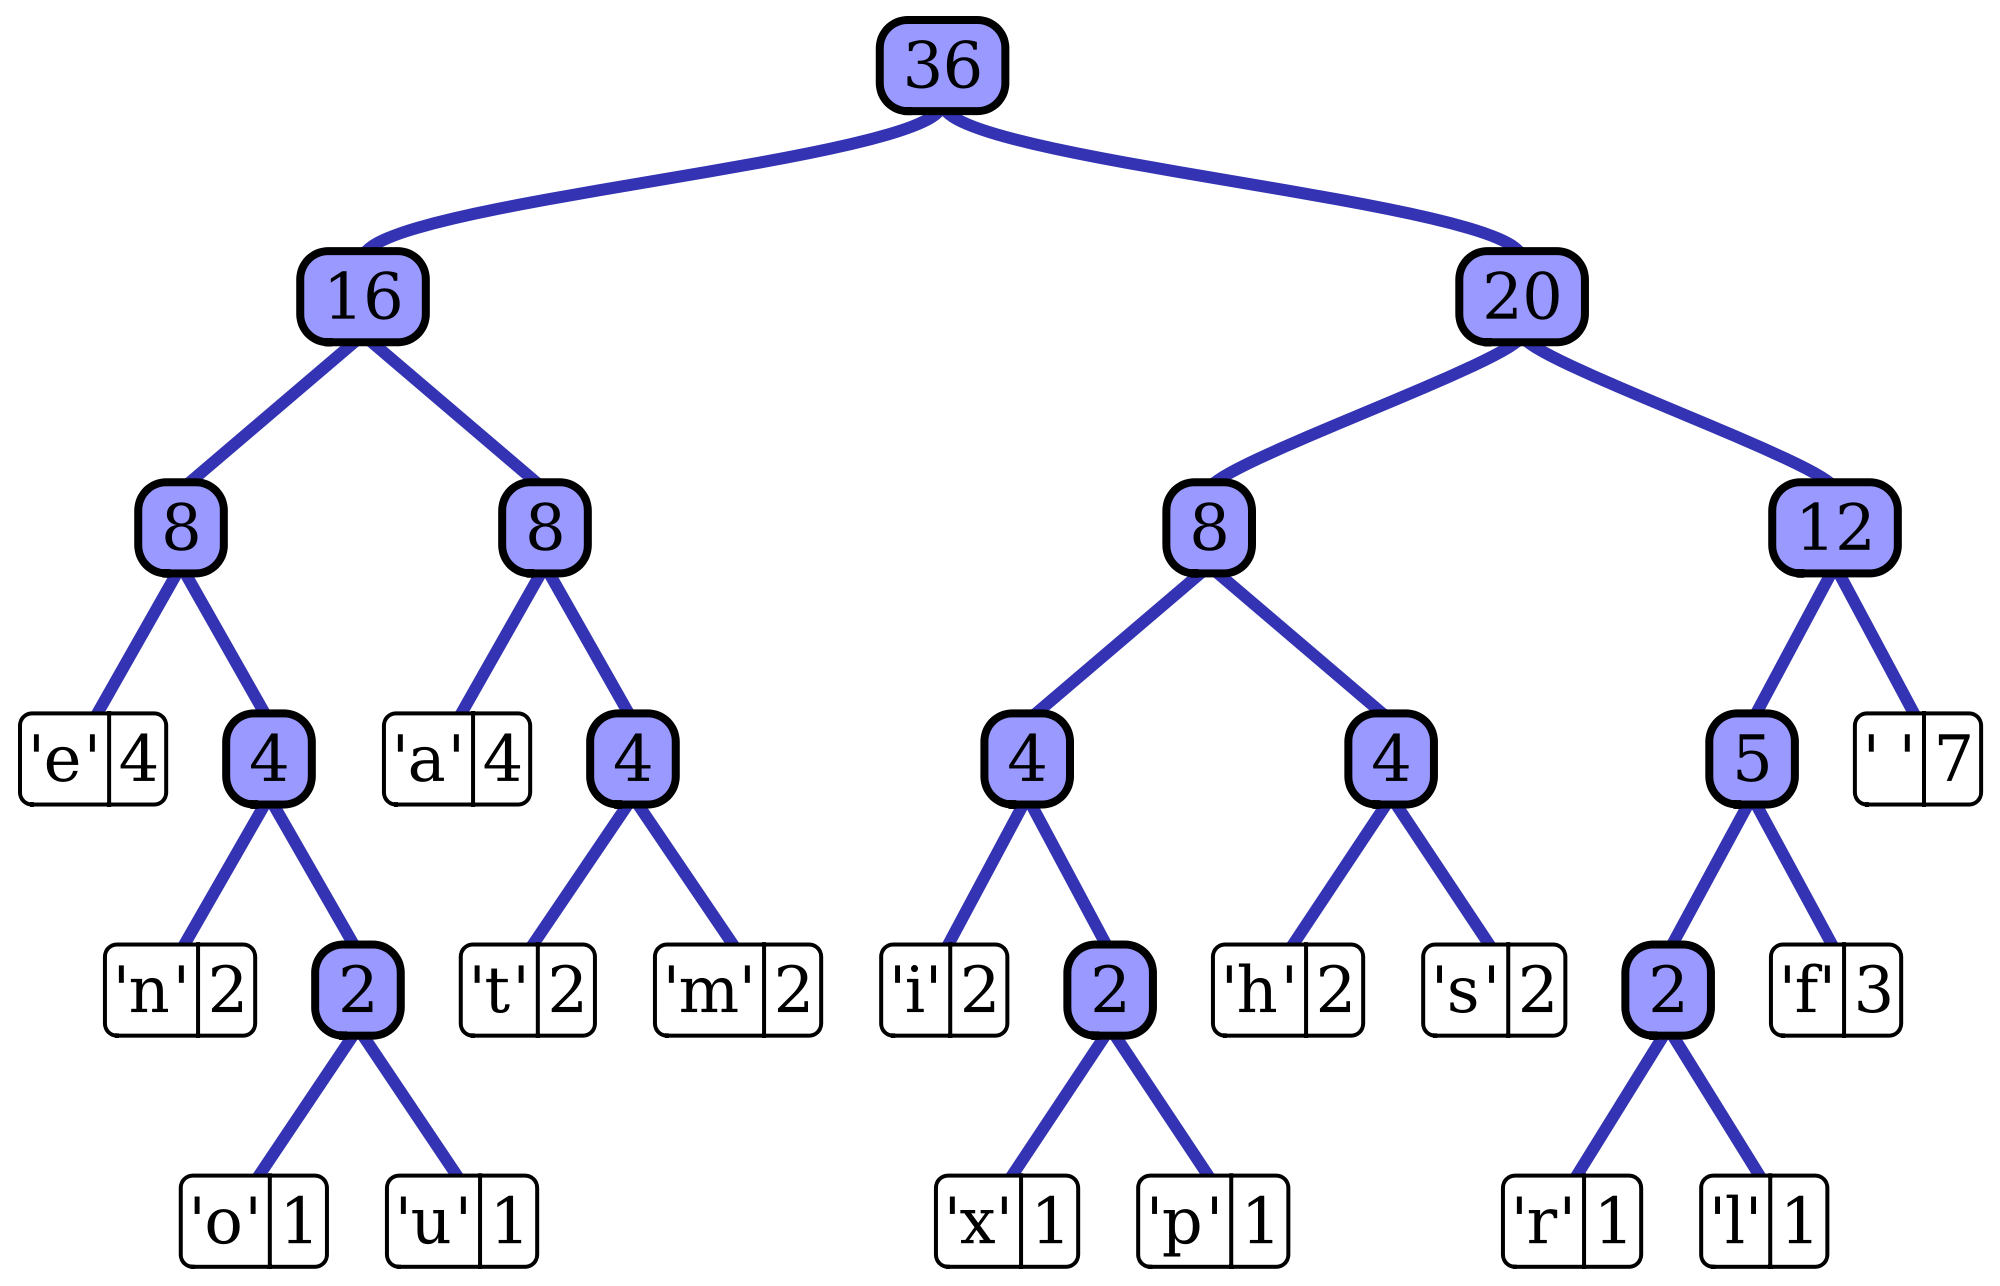
\includegraphics[width=\linewidth]{Billeder/Huffman_tree_2.png}
\caption{Huffman træ}
\label{fig:huffmantree}
\end{figure}

\begin{table}
\begin{center}
\begin{tabular}{|c|c|c|}
\hline
 \cellcolor{ForestGreen}\color{white}{\textbf{Tegn}} &  \cellcolor{ForestGreen}\color{white}{\textbf{Hyppighed}} & \cellcolor{ForestGreen}\color{white}{\textbf{Binær kode}} \\
\hline
space & 7 & 111 \\ 
\hline 
a & 4 & 010 \\ 
\hline 
e & 4 & 000 \\ 
\hline 
f & 3 & 1101 \\ 
\hline 
h & 2 & 1010 \\ 
\hline 
i & 2 & 1000 \\ 
\hline 
m & 2 & 0111 \\ 
\hline 
n & 2 & 0010 \\ 
\hline 
s & 2 & 1011 \\ 
\hline 
t & 2 & 0110 \\ 
\hline 
l & 1 & 11001 \\ 
\hline 
o & 1 & 00110 \\ 
\hline 
p & 1 & 10011 \\ 
\hline 
r & 1 & 11000 \\ 
\hline 
u & 1 & 00111 \\ 
\hline 
x & 1 & 10010 \\ 
\hline 
\end{tabular}
\caption{Hyppighed og kode af forskellige tegn}
\label{tab:huffmantable}
 \end{center}
\end{table}